%%++++++++++++++++++++++++++++++++++++++++++++++++++++++++++++++++++++++++++++
%%            INFORMATION
%%============================================================================
%%            Version
%%----------------------------------------------------------------------------
\def\CurrentVersionMain{\textit{V2.0}}
%%============================================================================
%%            Dokumentenklasse und Präambel
%%----------------------------------------------------------------------------
\documentclass[11pt,a4paper,oneside,bibliography=totocnumbered,toc=listofnumbered]{scrbook}
\usepackage[english,ngerman,naustrian]{babel}
\usepackage{./packages/WissensArbeitenFHWels}
\usepackage{./packages/WissensArbeitenFHWels-FrontseitenDE}     
\usepackage[utf8]{inputenc}
\usepackage{tikz}
\usepackage{matlab-prettifier}
\usepackage{tabularx}
%%++++++++++++++++++++++++++++++++++++++++++++++++++++++++++++++++++++++++++++
%%
%%++++++++++++++++++++++++++++++++++++++++++++++++++++++++++++++++++++++++++++
%%            DATEN/EINSTELLUNGEN für die WISSENSCHAFTLICHE ARBEIT
%%============================================================================
%%            Daten für die Arbeit
%%----------------------------------------------------------------------------
%% Titel der Arbeit:
\title{KSS4 Sensorkalibrierung und Kalman-Filter}
%%
%% Autor der Arbeit:
\author{Radlberger Paul / Gehmayr Emmanuel}
%%
%% Studiengang:
\studiengang{Robotic Systems Engineering}
%%
%% Typ des Dokuments:
\typDokument{Laborprotokoll}
% -) "Bachelorarbeit"
% -) "Masterarbeit"
% -) "Diplomarbeit"
% -) "Projektbericht"
%%
%% Art des Studiengangs:
\artStudiengang{Masterstudiengang}
% -) "Bachelorstudiengang"
% -) "Masterstudiengang"
% -) "Diplomstudiengang"
%%
%% Zu erlangender akademischer Grad:
%%\akademGrad{>>Akademischer Grad<<}
% -) "Bachelor of Science in Engineering (BSc)"
% -) "Master of Science in Engineering (MSc)"
% -) "Diplom-Ingenieurin für technisch-wissenschaftliche Berufe (Dipl.-Ing.)"
% -) "Diplom-Ingenieur für technisch-wissenschaftliche Berufe (Dipl.-Ing.)"
%%
%% Ort der Fakultät:
\studienort{Wels}
%%
%% Abgabemonat und Jahr:
\abgabemonat{Februar}
\abgabejahr{2020}
%%
%% Betreuer der Arbeit:
\betreuer{Ing. Michael Zauner BSc MSc}
%%
%% Stichwörter für die Arbeit:
%% (werden in die Metadaten des PDF's geschrieben)
\stichwoerter{Stichwort 1, Stichwort 2 Stichwort 3...}
%%
%% Unterschrift anzeigen: (ACHTUNG: Syntax wichtig!!!)
\ShowSignature{0mm}{22mm}{0.5}{No}		% Zeigt die Unterschrift auf der Eidest. Erklärung
% Syntax: {x-Position}{y-Position}{Skalierungsfaktor}{'Anzeigen:' Yes / No}
% Beispiel: \ShowSignature{0mm}{22mm}{0.5}{Yes}
% Datei mit dem Namen "Signature.png" muss im Grafik-Ordner vorhanden sein.
%%
%%	Eingefärbung der Links festlegen: (ACHTUNG: Syntax wichtig!!!)
\ColoredLinks{No}		% Eingefärbet Links(Abbildung, URL's, Literatur)
% Syntax: Yes / No
%%
%%============================================================================
%%            Einstellungen:
%%----------------------------------------------------------------------------
\Style{FHWels}				% Grundlegender Stil (nur 'FHWels' möglich)
\BibStyle{FHWelsNumericBrackets}	% Zitier-Stil auf Basis von 'BibLatex'
% Syntax:	-) FHWelsNumericBrackets (z.B.: [1])
%			-) FHWelsAlphabeticBrackets (z.B. [Meier, 2011])
\addbibresource{Bibliography.bib}	% Bibliography - Datei(en)
\graphicspath{{./Grafik/}}	% Festlegung des Unterordners für Abbildungen
\TabContent{1.4cm}			% Tabulatoreinrückung für das Inhaltsverzeichnis	
%%++++++++++++++++++++++++++++++++++++++++++++++++++++++++++++++++++++++++++++
%%
%%++++++++++++++++++++++++++++++++++++++++++++++++++++++++++++++++++++++++++++
%%            BEGINN der ARBEIT
%%============================================================================
\begin{document}
\selectlanguage{naustrian}	% Deutsche Sprache (Österreichpaket)	
%%============================================================================
%%            Titelseite & Eidesstattliche Erklärung
%%----------------------------------------------------------------------------
%% Titelseite
	\frontmatter				% römische Seitennummerierung				
	\pagenumbering{Roman}		% Großbuchstaben
	\titelseite
%%	
%%============================================================================
%%            Hauptteil der Arbeit
%%----------------------------------------------------------------------------
	\mainmatter					% arabische Seitennummierierung
	\clearpage
%%----------------------------------------------------------------------------
%% Einleitung	
	\chapter{Aufgabenstellung}
\label{sec: Aufgabenstellung}

\section{Laborübung 1 - Sensorkalibrierung}

Aufgabe der Laborübung ist es geeignete Messungen mit der IMU durchzuführen um diese aufgrund der gemessenen Signale kalibrieren zu können. Beim Kalibriervorgang sollten sowohl der Offsetfehler, als auch der Skalierungsfehler der einzelnen Sensorachsen korrigiert werden. Außerdem sollten zusammengehörige Sensordaten auf einen Referenzwert normiert werden (z.B. Beschleunigungssensoren in x-,y- und z-Achse auf den Wert $9,81\frac{m}{s^2}$), um ein korrektes Messergebnis gewährleisten zu können. Die Sensoren sollen auch bezüglich ihrer Varianz beurteilt werden.
Um die systematischen Fehler der Sensoren zu korrigieren sollen zunächst eine Reihe von Messungen durchgeführt werden. Alle Messungen sind in Tabelle \ref{tab:Messungen} gelistet.

\begin{table}[h]
	\centering
	\begin{tabular}{|p{2cm}|p{10.6cm}|p{2cm}|}
		\hline
		\rowcolor{lightgray}\textbf{Messung} & \textbf{Durchführung} & \textbf{Dauer} \\
		\hline
		1	&Messung der Erdbeschleunigung in positive x-Richtung			& 30 s\\
		\hline
		2	&Messung der Erdbeschleunigung in positive y-Richtung			& 30 s\\
		\hline
		3	&Messung der Erdbeschleunigung in positive z-Richtung			& 30 s\\
		\hline
		4	&Messung der Erdbeschleunigung in negative x-Richtung			& 30 s\\
		\hline
		5	&Messung der Erdbeschleunigung in negative y-Richtung			& 30 s\\
		\hline
		6	&Messung der Erdbeschleunigung in negative z-Richtung			& 30 s\\
		\hline
		7	&Messung des Magnetfeldes in x-, y- und z-Richtung – Sensor wird dabei um alle Achsen zufällig rotiert	& 60 s\\
		\hline
		8	&Messung der Drehraten um die x-, y- und z-Achse – Sensor wird dabei nicht bewegt!	& 30 s\\
		\hline
	\end{tabular}
	\caption{Messungen zur Sensorkalibrierung}
	\label{tab:Messungen}
\end{table}

\subsection{Abgleich Beschleunigungssensor}
Für die Kalibrierung des Beschleunigungssensors werden die Messungen 1-6 aus Tabelle \ref{tab:Messungen} herangezogen. Als Referenzwert für die Kalibrierung wird die Erdbeschleunigung $g=9,81\frac{m}{s^2}$) verwendet, welche stets konstant ist und bei entsprechender Orientierung der IMU immer nur entlang einer der drei Koordinatenachsen wirkt. Aus jeweils einem Paar von Messungen (z.B. aus den Messungen 1 und 4) können a\textsubscript{min} und a\textsubscript{max} berechnet werden, wobei a\textsubscript{min} und a\textsubscript{max} jeweils aus dem Mittelwert der Messfolge jener Koordinatenachse sind. Anschließend kann der durchschnittliche Endausschlag bei voller Erdbeschleunigung a\textsubscript{peak} ermittelt werden.
\begin{align}
	a_{peak}=\frac{\vert{a_{min}}\vert+\vert{a_{max}}\vert}{2}
	\label{eq: a_peak}
\end{align}
Über den Referenzwert g kann anschließend der Skalierungsfaktor für die Normierung (s\textsubscript{norm}) berechnet werden.
\begin{align}
	s_{norm}=\frac{g}{a_{peak}}
	\label{eq: s_norm}
\end{align}
Der entsprechende normierte Offsetabgleich lässt sich wie folgt berechnen berechnen.
\begin{align}
	a_{off}=(a_{max}-a_{peak})\cdot{s_{norm}}
	\label{eq: a_off}
\end{align}
Der korrigierte Wert a\textsubscript{ist} kann aus dem Messwert a\textsubscript{m} berechnet werden.
\begin{align}
	a_{ist}=a_m\cdot{s_{norm}}-a_{off}
	\label{eq: a_ist}
\end{align}
Diese Vorgehensweise ist für jede Achse durchzuführen.

\subsection{Abgleich Magnetometer}
Für die Kalibrierung des Magnetometers wird Messung 7 aus Tabelle \ref{tab:Messungen} herangezogen. Als Referenzwert für die Kalibrierung kann die mittlere Stärke des Erdmagnetfeldes in Mitteleuropa m\textsubscript{e} verwendet werden. Dies beträgt 48 μT. Aus jeweils der Messfolge der jeweiligen Koordinatenachse kann m\textsubscript{min} und m\textsubscript{max} bestimmt werden, wobei m\textsubscript{min} und m\textsubscript{max} über eine Maximalwertsuche bzw. eine Minimalwertsuche bestimmt wird. Analog zu den für den Beschleunigungssensor durchgeführten Berechnungen lassen sich anschließend auch für das Magnetometer die Kalibrierwerte über die nachfolgenden Formeln berechnen.
\begin{align}
	m_{peak}=\frac{\vert{m_{min}}\vert+\vert{m_{max}}\vert}{2}
	\label{eq: m_peak}
\end{align}
\begin{align}
	m_{norm}=\frac{m_e}{m_{peak}}
	\label{eq: m_norm}
\end{align}
\begin{align}
	m_{off}=(m_{max}-m_{peak})\cdot{s_{norm}}
	\label{eq: m_off}
\end{align}
\begin{align}
	m_{ist}=m_m\cdot{s_{norm}}-m_{off}
	\label{eq: m_ist}
\end{align}

\subsection{Abgleich Gyroskope}
Für die Kalibrierung des Gyroskops wird die Messung 8 aus Tabelle \ref{tab:Messungen} herangezogen. Da keine definierte Drehbewegung um eine Koordinatenachse im Labor durchgeführt werden kann, kann kein Referenzwert für das Gyroskop bestimmt werden. Aus diesem Grund kann die Skalierung des Gyroskops nicht kalibriert werden. Beim Gyroskop kann lediglich ein Offsetabgleich durchgeführt werden. Da sich bei den Messungen 8 der Sensor in Ruhelage befand, muss die Winkelgeschwindigkeit gleich Null sein. Durch Mittelwertbildung über die Messwertfolgen der Winkelgeschwindigkeiten können die Offsetwerte aller Achsen berechnet werden.
\begin{align}
	\omega_{ist}=\omega_m-\omega_{off}
	\label{eq: omega_ist}
\end{align}

\subsection{Temperaturabgleich}
Es wird eine Messreihe der kalibrierten Werte aufgenommen. Dabei wird der Sensor auf eine maximale Temperatur von 80 °C erwärmt. Im Anschluss können alle Einzelsensorwerte über der Temperatur dargestellt werden und eine Ausgleichsfunktion bestimmt werden.

\subsection{Bestimmung der Varianz der einzelnen Sensoren}
Für Bestimmung der Varianz kann die Messung 8 aus Tabelle \ref{tab:Messungen} herangezogen werden.

\section{Laborübung 2 - Kalman Filter}
Es soll ein Kalman-Filter in Matlab implementiert werden:
\begin{enumerate}
	\item	Prädiktor-Schritt: \\
	Bestimmung des Neigungswinkel mit Hilfe des Gyroskops.
	\begin{align}
		\bar{\mu}_{t+1}=A\cdot{\mu_t}+B\cdot{u_{t+1}} \\
		\bar{\Sigma}_{t+1}=A\cdot{\Sigma_t}\cdot{A^T}+\Sigma_u
		\label{eq: Predictor}
	\end{align}
	\item	Korrektur-Schritt: \\
	Die Korrektur des Neigungswinkel wird mit Hilfe des berechneten Winkels der Beschleunigungssensoren durchgeführt.
	\begin{align}
		K_{t+1}=\bar{\Sigma}_{t+1}\cdot{H^T}\cdot{(H\cdot{\bar{\Sigma}_{t+1}}\cdot{H^T}+\Sigma_z)^{-1}} \\
		\mu_{t+1}=\bar{\mu}_{t+1}+K_{t+1}\cdot{(z_{t+1}-H\cdot{\bar{\mu}_{t+1}})} \\
		\Sigma_{t+1}=(I-K_{t+1}\cdot{H})\cdot{\bar{\Sigma}_{t+1}}
		\label{eq: Corrector}
	\end{align}
\end{enumerate}
Die Matrizen für die Drehbewegung um eine Achse können wie folgt eingegeben werden (siehe Skript):

\begin{equation*}
A = 
\begin{bmatrix}
1 & -dt \\
0 & 1   \\
\end{bmatrix}
\end{equation*}
\begin{equation*}
B = 
\begin{bmatrix}
dt \\
0  \\
\end{bmatrix}
\end{equation*}
\begin{equation*}
H = 
\begin{bmatrix}
1 & 0 \\
\end{bmatrix}
\end{equation*}
\begin{equation*}
I = 
\begin{bmatrix}
1 & 0 \\
0 & 1 \\
\end{bmatrix}
\end{equation*}

Um eine Überprüfung der Funktionalität des zu implementierenden Kalman-Filters durchzuführen zu können, sollen IMU-Messungen, wie in Tabelle  \ref{tab:Messungen} angegeben, aufgenommen werden. Es werden zuerst Messungen aufgenommen, in welcher nur rotatorische Bewegungen getätigt wurden (Messung 1 - 3). In Messung 4 soll gezeigt werden, dass störende Querbeschleunigungen kompensiert werden können.

\begin{table}[h]
	\centering
	\begin{tabular}{|p{2cm}|p{10.6cm}|p{2cm}|}
		\hline
		\rowcolor{lightgray}\textbf{Messung} & \textbf{Durchführung} & \textbf{Dauer} \\
		\hline
		1	&Rotation um die x-Achse (±45 °)		& 30 s\\
		\hline
		2	&Rotation um die y-Achse (±45 °)		& 30 s\\
		\hline
		3	&Rotation um die z-Achse (±45 °)		& 30 s\\
		\hline
		4	&Rotation um die x-Achse und gleichzeitiges Bewegen in die positive und negative y-Richtung			& 30 s\\
		\hline
	\end{tabular}
	\caption{Messungen zur Überprüfung des Kalman- Filters}
	\label{tab:Angabe Kalman-Filter}
\end{table}

%%----------------------------------------------------------------------------
%% Hauptkapitel 1
	\chapter{Erfassung der Messwerte}
\label{sec: Erfassung der Messwerte}

\begin{figure}[h]
	\centering
	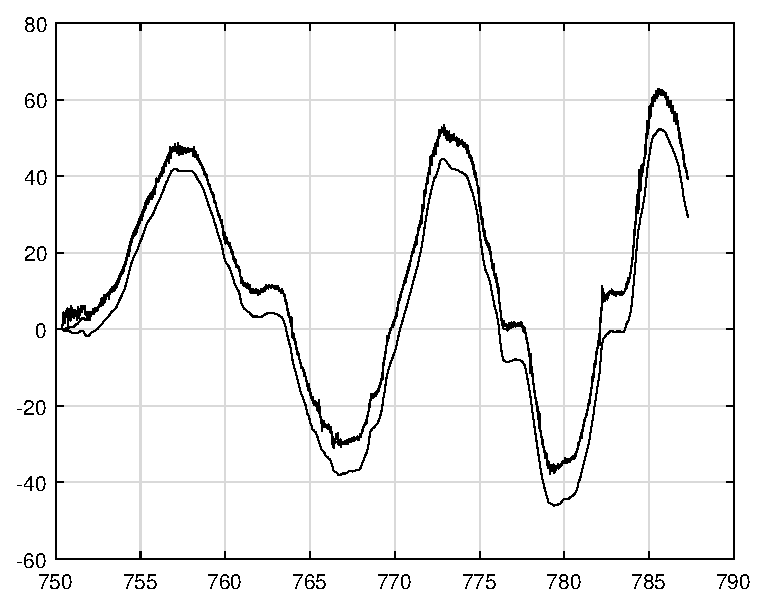
\includegraphics[width=1\textwidth]{Matlab/KalmanXRotation.eps}
	\caption{Grafik1}
	\label{fig: Grafik1}
\end{figure}


\begin{figure}[h]
	\centering
	\lstinputlisting{Matlab/Kalman.m}
	\caption{Grafik2}
	\label{fig: Grafik2}
\end{figure}
%%----------------------------------------------------------------------------
%% Hauptkapitel 2
	%\chapter{Stapler}
\label{sec: Stapler}

Unabhängig von der Navigation muss der Stapler verschiedene Aktionen ausführen können, welche wiederum Sensorik benötigen. Die Aufgaben, welcher der Stapler zu erfüllen hat, sind im folgenden aufgezählt:
\begin{itemize}
	\item Fortbewegung
	\item Heben von Lasten
	\item Lenken
\end{itemize}	
\begin{figure}[h]
	\centering
	\includegraphics[width=0.50\textwidth]{Stapler Sensorpositionen.png}
	\caption{Stapler Sensorpositionen}
	\label{fig: Stapler Sensorpositionen}
\end{figure}

\section{Fortbewegung}\label{sec:Fortbewegung}
Der Stapler hat 4 Räder, welche auf 2 mechanischen Achsen montiert sind (vorne und hinten). Dabei wird Achse 1 durch einen Motor angetrieben und Achse 2 läuft mit Achse 1 mit. Um dies sensorisch abzudecken, wird auf der angetriebenen Achse ein Inkrementalgeber verbaut. Dieser dient einerseits zur Überwachung und Regelung der Geschwindigkeit und andererseits für die odometrische Bestimmung der Pose. Die Geberdaten werden direkt an die zentrale Steuerungseinheit des Stapler und an die Antriebe übertragen. Optional kann auf der nicht-angetriebenen Achse ein zusätzlicher Inkrementalgeber montiert werden. Mit der zusätzlichen Information der Geschwindigkeit des 2 Inkrementalgeber kann eine Rutsch oder Schleifbewegung detektiert werden. Mit dieser Information kann die Pose der odometrischen Berechnung korrigiert werden.

\section{Heben von Lasten}\label{sec:Heben von Lasten}
Nimmt der Stapler eine Last auf, so verändert sich der Schwerpunkt des gesamten Fahrzeugs, was im schlimmsten Fall zum Kippen führen kann. Aus diesem Grund ist die Längsachse kippbar gelagert, wodurch der Schwerpunkt wieder richtung Fahrzeugmitte korrigiert werden kann. Der Stapler ist konstruktiv so konstriert, dass mit einem konstantem Kippwinkel jede Last befördert und gehobten werden kann. Damit ist nur eine, immer gleichbleibende Kippbewegung auszuführen und die aktuelle Kipplage mithilfe von Endschaltern zu erfassen. Um die Kipplage sicher zu erfassen, werden pro Endlage 2 Sensoren verbaut. Die 2 Position werden Transport- und Ladeposition genannt.
\begin{figure}[h]
	\centering
	\includegraphics[width=0.50\textwidth]{Stapler Kippbewegung.png}
	\caption{Stapler Kippbewegung}
	\label{fig: Stapler Kippbewegung}
\end{figure}

\section{Lenken}\label{sec:Lenken}
Durch Neigen der Längsachse kann der Stapler in verschiedene Richtungen fahren und dadurch Lenkbewegungen ausführen. Durch den Aufbau des Staplers ist eine Drehung nur in Verbindung mit einer Fortbewegung möglich. Die Neigung der Längsachse erfolgt durch einen Motor, welcher eine vorgegebene Winkel- Sollposition anfährt. Um die aktuelle Lage der Achse zu erfassen, wird ein Absolutwertgeber am Drehgelenk angebracht. Durch den Einsatz eines Absolutwertgebers kann die Istposition des Sensors nicht verschwinden und beim Einschalten des Staplers muss die aktuelle Position nicht referenziert werden.
\begin{figure}[h]
	\centering
	\includegraphics[width=0.50\textwidth]{Stapler Lenkbewegung.png}
	\caption{Stapler Lenkbewegung}
	\label{fig: Stapler Lenkbewegung}
\end{figure}
%%----------------------------------------------------------------------------
%% Zusammenfassung
	%\input{Text/0501-Zusammenfassung}
%%----------------------------------------------------------------------------
%% Abkürzungsverzeichnis[optional]
	\clearpage
	\input{Text/9001-Abkuerzungen}
%%----------------------------------------------------------------------------
%% Abbildungsverzeichnis [optional]
	\clearpage
	\input{Text/9003-Abbildungsverzeichnis}
%%----------------------------------------------------------------------------
%% Literaturverzeichnis
	\clearpage
	\chapter{Literaturverzeichnis}
\label{sec: Bibliography}
Nachstehend finden Sie zwei Muster-Literaturverzeichnisse, die die wichtigsten Arten von Veröffentlichungen abdecken (reine Internet-Quelle, Norm, Monografie, Aufsatz in einem Sammelband, technische Regel, Zeitschriftenaufsatz). Informationen zu weiteren Publikationstypen finden Sie für das Deutsche in der unten genannten ONR~12658, für das Englische in der unten genannten ISO~690. Beide Regelwerke sind in der Bibliothek des FH-OÖ-Campus Wels einsehbar.

\section{Literaturverzeichnis bei Nutzung von Quellenangaben im Text (PDK) oder in der Fußnote (MEWI)}
\printbibliography[heading=none,env=bibliographyAlpha]
\nocite{*}

\section{Literaturverzeichnis bei Nutzung von Quellenangaben in Form von Zahlen in eckigen Klammern (VTP, MEWI, MKT)}
\printbibliography[heading=none]

\newpage
\subsection*{Erscheinungsbild}
Das Aussehen des Literaturverzeichnisses hängt von der Zitierweise ab, die Sie in Ihrer wissenschaftlichen Arbeit anwenden müssen [siehe Abschnitt \ref{sec: ZitierStil} auf S. \pageref{sec: ZitierStil}].

\subsection*{Gliederung}
Das Literaturverzeichnis kann bei Bedarf in folgende Unterkapitel untergliedert werden:
\begin{itemize}
	\item	Primärliteratur 
	\item	Sekundärliteratur 
	\item	Tertiärliteratur
\end{itemize}

\subsection*{Literaturrecherche}
Auf den Internetseiten der Bibliothek des FH-OÖ-Campus Wels finden Sie eine sehr übersichtliche Liste mit zahlreichen Links zu:
\begin{itemize}
	\item	elektronischen Zeitschriften
	\item	Datenbanken
	\item	zahlreichen Bibliotheken
	\item	Katalogen des Buchhandels
	\item	Patentgesellschaften
\end{itemize}
Die MitarbeiterInnen der Bibliothek unterstützen Sie gerne bei der Literaturrecherche.


%%============================================================================	
\end{document}
%%++++++++++++++++++++++++++++++++++++++++++++++++++++++++++++++++++++++++++++